%-------------------------------------------------------------------------------
\section{Motivation}
%-------------------------------------------------------------------------------
\begin{figure}[h]
\center{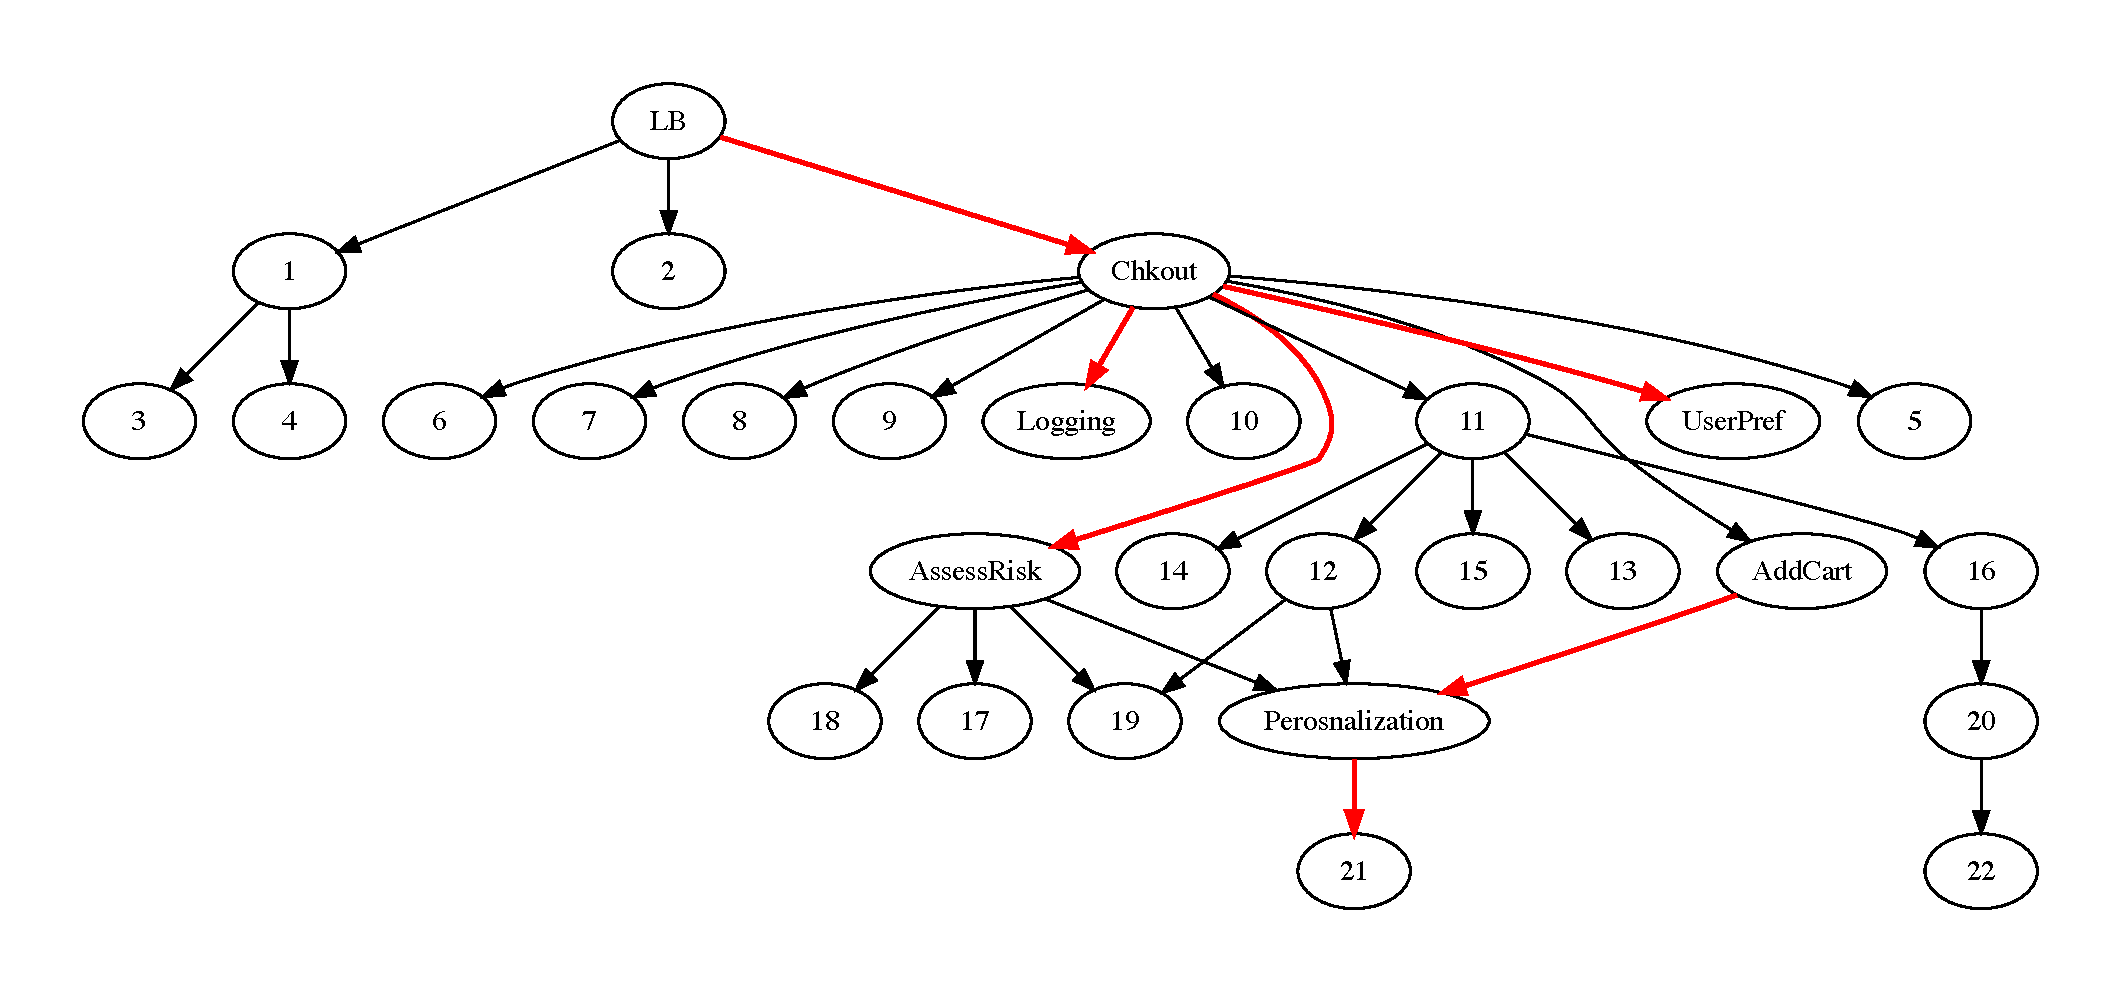
\includegraphics[scale=0.25]{anon_adrbk_fail.pdf}}
\caption{Example graph drawn from trace of a failed interaction. The red lines indicate that the callee has returned an error message to the caller}
\label{Failed_ex}
\end{figure}

In a failed interaction, such as the one seen in Figure~\ref{Failed_ex}, all the services which are not successful will be altering. The job of an SRE in this situation is to find the cause of the failure by:
\begin{itemize}
\item Figuring out which of the alerts are smokescreens to be ignored. \newline
Some services that are called as part of the interaction which provide useful functionality, but the failure of which can be tolerated by the system, can be thought of as nice-to-have services. Alerts from such services may be safely ignored, the key is knowing which services these are and also how they interact with other services. 
\item Using domain knowledge about the dependencies between services to know which alerts are the result of transitive dependencies and must be ignored. \newline
As an example, the load balancer (LB) in the figure will be alerting. An intelligent observer would conclude that since checkout (Chkout) has multiple downstream alerts, the alerts at LB are probably a result of the error being propagated up and try to dig deeper into one of the downstream alerts that look promising.
\item Determining if the absence of some services caused the failure \newline
Failures are sometimes caused by services which are required failing or a fallback path not being taken. Details of a network connection failure or time out in attempting to connect to downstream services might be buried deep in the trace. Even after we find them, figuring out the path that should have been taken but wasn't can be challenging. 
\end{itemize}
The question we ask is: How we can encode knowledge gained from witnessing successful executions to provide hints of possible causes when an execution fails? This is the crux of the trace forensics problem we touched upon in the introduction.
